% -----------------------------------------------
% Template for ISMIR Papers
% 2023 version, based on previous ISMIR templates

% Requirements :
% * 6+n page length maximum
% * 10MB maximum file size
% * Copyright note must appear in the bottom left corner of first page
% * Clearer statement about citing own work in anonymized submission
% (see conference website for additional details)
% -----------------------------------------------

\documentclass{article}
\usepackage[T1]{fontenc} % add special characters (e.g., umlaute)
\usepackage[utf8]{inputenc} % set utf-8 as default input encoding
\usepackage{ismir,amsmath,cite,url}
\usepackage{graphicx}
\usepackage{color}

% inserted packages, remove before submission
\usepackage{booktabs} % for better-looking tables
\usepackage[bookmarks=false,hidelinks]{hyperref}
\usepackage{tabularx}
\usepackage{float}
\usepackage{xcolor}
\usepackage{multicol}
\usepackage{multirow}
\usepackage{stfloats} % table positions
\usepackage{caption}
\usepackage{siunitx}
% \usepackage[justification=centering]{caption}
% \usepackage[width=.75\textwidth,justification=centering]{caption}

\newcommand{\rephr}[1]{{\color{black!50} #1}}
\newcommand{\todo}[1]{{\color{blue!50} #1}}
\newcommand{\ph}[1]{{\color{violet} #1}}
\newcommand{\gw}[1]{{\color{teal} G: #1}}

\usepackage{xspace}
% \newcommand{\repo}{\texttt{\_\_link\_\_}\xspace}
% \newcommand{\repo}{\texttt{https://github.com/CPJKU/musically\_informed\_evaluation}}
\newcommand{\repo}{\url{https://github.com/CPJKU/mpteval}}


\usepackage{lineno}
% \linenumbers

% Title. Please use IEEE-compliant title case when specifying the title here,
% as it has implications for the copyright notice
% ------
\title{Towards musically informed evaluation \\ of piano transcription models}
% On the reliability of piano transcription models for 

% Note: Please do NOT use \thanks or a \footnote in any of the author markup

% Single address
% To use with only one author or several with the same address
% ---------------
%\oneauthor
% {Names should be omitted for double-blind reviewing}
% {Affiliations should be omitted for double-blind reviewing}

% Two addresses
% --------------
%\twoauthors
%  {First author} {School \\ Department}
%  {Second author} {Company \\ Address}

% Three addresses
% --------------\input{ISMIR2021_paper.tex}

% \threeauthors
%   {First Author} {Affiliation1 \\ {\tt author1@ismir.edu}}
%   {Second Author} {\bf Retain these fake authors in\\\bf submission to preserve the formatting}
%   {Third Author} {Affiliation3 \\ {\tt author3@ismir.edu}}

% Four or more addresses
% OR alternative format for large number of co-authors
% ------------
\multauthor
{Patricia Hu$^1$ \hspace{0.54cm} Luk\'a\v{s} Samuel Mart\'ak$^{1,2}$ \hspace{0.54cm} Carlos Cancino-Chac\'on$^1$ \hspace{0.54cm} Gerhard Widmer$^{1,2}$} 
{
$^1$ Institute of Computational Perception, Johannes Kepler University Linz, Austria\\
$^2$ {LIT AI Lab, Linz Institute of Technology, Austria}\\
{\tt patricia.hu@jku.at}
}

% For the author list in the Creative Common license, please enter author names. 
% Please abbreviate the first names of authors and add 'and' between the second to last and last authors.
\def\authorname{P. Hu, L. Mart\'ak, C. Cancino-Chac\'on and G. Widmer}
% \def\authorname{Hu et al.} % saves space...

% Optional: To use hyperref, uncomment the following.
%\usepackage[bookmarks=false,pdfauthor={\authorname},pdfsubject={\papersubject},hidelinks]{hyperref}
% Mind the bookmarks=false option; bookmarks are incompatible with ismir.sty.

\sloppy % please retain sloppy command for improved formatting

\begin{document}

%
\maketitle
%
\begin{abstract} % 150-200 words
%%%%%% version 2
Automatic piano transcription models are typically evaluated using simple frame- or note-wise information retrieval (IR) metrics. Such benchmark metrics do not provide insights into the transcription quality of specific musical aspects such as articulation, dynamics, or rhythmic precision of the output, which are essential in the context of expressive performance analysis.
Furthermore, in recent years, MAESTRO has become the de-facto training and evaluation dataset for such models. However, inference performance has been observed to deteriorate substantially when applied on out-of-distribution data, thereby questioning the suitability and reliability of transcribed outputs from such models for specific MIR tasks.
In this work, we investigate the performance of three state-of-the-art piano transcription models in two experiments. In the first one, we propose a variety of musically informed evaluation metrics which, in contrast to the IR metrics, offer more detailed insight into the musical quality of the transcriptions.
In the second experiment, we compare inference performance on real-world and perturbed audio recordings, and highlight musical dimensions which our metrics can help explain.
% In the second experiment, we simulate real-world recording environments using different acoustic conditions and noise levels, and again investigate the musical quality of the transcribed results using our proposed metrics.
Our experimental results highlight the weaknesses of existing piano transcription metrics and contribute to a more musically sound error analysis of transcription outputs.
\end{abstract}

%%%%%%%%%%%%%%%%%%%%%%%%%%%%%%%%%%%%%%%%%%%%%%%%%%%%%%%%%%%%%%%%
%%%%%%%%%%%%%%%%%%%%%%%%%%%%%%%%%%%%%%%%%%%%%%%%%%%%%%%%%%%%%%%%
%%%%%%%%%%%%%%%%%%%%%%%%%%%%%%%%%%%%%%%%%%%%%%%%%%%%%%%%%%%%%%%%

\section{Introduction}\label{sec:introduction}
% Automatic music transcription (AMT) refers to the task of converting audio signals into symbolic music representations. The target output format can be a full symbolic score including quantized rhyhtm, time signature and pitch spelling information, in which case the conversion task is referred to as Complete Music Transcription (CMT),  This variant of the transcription task is relatively less studied, with most current methods focusing on the problem of multi-pitch detection, producing a mid-level physical MIDI-like representation, describing notes in terms of their onset and offset times, pitch and velocity \cite{hawthorne2017onsets, kong2021highresolution, hawthorne2021sequence}. For the remainder of this article, we will therefore refer to this audio-to-MIDI(-like) conversion task as AMT.

Automatic Music Transcription (AMT) refers to the task of converting audio signals into symbolic music representations. The target output format can be a full symbolic score including quantized rhythm, time signature and pitch spelling information, or a mid-level physical MIDI(-like) representation, describing notes in terms of their onset and offset times, pitch and velocity \cite{hawthorne2017onsets, kong2021highresolution, hawthorne2021sequence}.

AMT methods are typically evaluated using information retrieval (IR) metrics like precision, recall and F1 score \cite{bay2009evaluation}. These IR metrics can be computed at the level of frames, by comparing binary piano roll-like matrices, or at the level of note lists, by comparing notes in terms of their onset, offset, pitch and/or velocity attributes. Each error (i.e. misplaced frame or note activity) has equal weight, resulting in limited explanatory power of these metrics with respect to the underlying musical material \cite{hawthorne2017onsets, ycart2020investigating}.

As in many other areas in MIR, the current state-of-the-art is defined by deep neural networks \cite{lu2023multitrack, hawthorne2021sequence, kong2021highresolution}. To a large extent, this progress has been enabled by the release of the MAESTRO dataset \cite{hawthorne2019enabling}, which made well-aligned audio-MIDI piano performance data available
% to the community
on a large scale. The most up-to-date version of the MAESTRO dataset\footnote{https://magenta.tensorflow.org/datasets/maestro} contains close to 200 hours of performance data from close to 1300 recordings of Western classical piano repertoire. State-of-the-art piano transcription systems achieve beyond 90\% frame-level, or 80\% note-level F1 scores on its test split \cite{hawthorne2019enabling, kong2021highresolution, hawthorne2021sequence, gardner2021mt3}, and have led to the release of large-scale transcribed solo piano performance datasets \cite{kong2020giantmidi, zhang2023atepp}.
%{
% model  |  frame  |  note_on  | note_on_off  |  note_on_off_vel
% OAF    |  90.15  |    95.32  |    80.50     |     77.54
% OaF r  |  85.27  |    -      |    59.31     |     56.95
% Kong   |  98.62  |    96.72  |    82.47     |     80.92
% Kong r |  90.02  |    -      |    82.15     |     80.41
% T5     |    -    |    96.01  |    83.94     |     82.75
% T5 r   |  65.52  |    -      |    59.68     |     58.96

% model  |  frame  | note_on   | note_on_off  |  note_on_off_vel
% OAF    |  90.15  |    95.32  |    80.50     |     77.54
% Kong   |  98.62  |    96.72  |    82.47     |     80.92
% T5     |    -    |    96.01  |    83.94     |     82.75


%}

Although these results are impressive, we believe that two important aspects have been largely overlooked: first, the validity and (lack of) explanatory power of the standard evaluation metrics with respect to musically relevant information, and second, the reliability of these transcription models on out-of-distribution data. In this work, we address the first problem by proposing a set of musically informed evaluation metrics that support a more nuanced understanding of piano transcription errors. The metrics are intended to be used in the context of computational performance studies,
% of Western classical solo piano work, 
and therefore focus on musical dimensions that are commonly studied in the context of expressive piano performance analysis and generation. We demonstrate our metrics on a subset of the MAESTRO dataset, which we transcribe using three state-of-the-art transcription models. In particular, we contrast the performance of these models, as evaluated with the standard IR metrics, with their performance on musical dimensions such as timing, articulation and dynamics which we can evaluate using our set of musically informed metrics. 

Then, to elucidate the second problem, we re-record a subset of the MAESTRO dataset on a Yamaha Disklavier grand piano and further manipulate the audio recordings by adding different levels of noise and reverberation. An analysis of the outputs of the pre-trained transcription models on these recordings provides some detailed insights into the lack of generalization on out-of-distribution data. We make our set of metrics, data and all experimental results available at \repo.

% \gw{The following paragraph can easily go. The paper structure is totally obvious from the section headings and from the introduction.}
% The remainder of the paper is organized as follows: Section \ref{sec:related_work} discusses the benchmark evaluation metrics and datasets. In Section \ref{sec:musical_metrics}, we give an overview of our musically informed metrics. Next, Section \ref{sec:data} describes the data we use in our experiments. In Section \ref{sec:demonstration} we then demonstrate and compare our musical evaluation metrics to the standard ones. Then in Section \ref{sec:ood_inference} we illustrate the problem of out-of-distribution inference on re-rerecorded MAESTRO, and artificially manipulated audio data. We conclude our study in Section \ref{sec:conclusion} with a discussion of future research directions.

\section{Related Work}\label{sec:related_work}

This section briefly reviews the standard IR evaluation metrics along with criticism related to these, followed by a description of the benchmark datasets typically used for evaluating transcription methods.

Precision, recall and F1 score are the standard evaluation metrics used in AMT \cite{hawthorne2017onsets, kong2021highresolution, hawthorne2021sequence, bay2009evaluation}. They can be computed either at the level of frames or at the level of notes. Frame-level evaluation compares two binary piano roll matrices $M, \hat{M} \in \{0, 1\}^{p \times t}$, where $p$ defines the pitch range and $t$ the temporal resolution of a frame (typically 10ms \cite{bay2009evaluation}). Both $M$ and $\hat{M}$ are sparse matrices where 1 at a given index $p,t$ indicates a note with pitch $p$ is active at time frame $t$. True positives (TP) are then counted for frames in which $M_{p,t} = \hat{M}_{p,t} = 1$, false positives (FP) for frames where $M_{p,t} = 0$ but $\hat{M}_{p,t} = 1$, and false negatives (FN) for frames where $M_{p,t} = 1$ but $\hat{M}_{p,t} = 0$. Precision, recall and F1 score are then calculated on these counts. 
% computed as defined in Eqs. \ref{eq:IR_metrics}.
% \gw{I think these formulas can easily go. Everybody knows P, R, F1. "Precision, recall and F1 score are ." would do nicely.}

% \begin{equation}
% \begin{aligned}
% P & =\sum_{t=0}^{T-1} \frac{T P[t]}{T P[t]+F P[t]} \\
% R & =\sum_{t=0}^{T-1} \frac{T P[t]}{T P[t]+F N[t]} \\
% F_1 & =\frac{2 \cdot P \cdot R}{P+R}
% \label{eq:IR_metrics} 
% \end{aligned}
% \end{equation}

Note-level metrics are computed by comparing lists of notes, in which each note is described by a tuple describing the onset, offset, pitch, and (where predicted) velocity. Note-based metrics can be based on onset information only, onset and offset information (i.e., note durations), or on predicted onset, offset and velocity. In onset-only note evaluation, a note is considered correct if its onset falls within a $\pm$50 ms threshold of its respective target onset. For onset-and-offset note-level evaluation, the note offset must fall within the greater of either an offset tolerance threshold of $\pm$50 ms, or a duration threshold 20\% of the ground truth duration \cite{bay2009evaluation}. If velocity is included in the evaluation, an estimated note is considered correct if its velocity (after some normalization and rescaling operations) falls within a 0.1 tolerance threshold of the velocity of the corresponding reference note \cite{hawthorne2017onsets}.

% metrics validitiy
The need for better (i.e., musically or perceptually sound) transcription metrics has been expressed by various researchers before. Hawthorne et al.~\cite{hawthorne2017onsets} point out that frame- and onset-only note-level evaluation does not sufficiently capture musically relevant information. Similarly, Ycart et al. \cite{ycart2020investigating} and Daniel et al. \cite{daniel2008perceptually} focus on the problem of perceptual saliency of different kinds of transcription errors and each propose a new, perceptually (more) valid transcription metric. Finally, McLeod and Steedman \cite{mcleod2018evaluating} focus on the problem of audio-to-score transcription and propose a new metric that jointly evaluates voice separation, metrical alignment, note value detection and harmonic analysis along with multi-pitch detection.

% dataset diversity
% { ----------- DATASET DIVERSITY -----------
% MAESTRO Dataset
% composers from 17th-20th century
% alignments were created by minimizing the CQT frames distance between audio and synthesized MIDI using FluidSynth
% MIDI and Audio Edited for Synchronous TRacks and Organization
% v-1 : 172 hrs, ~3ms alignment bw note labels and audio waveforms
% --- each composition is unique to one split 
% --- ratio 80/10/10 : globally and within each composer
% --- for val and test : more repertoire diversity; for train : more performer diversity
% v-3 : +26hrs/ 92 performances
% --- includes sostenuto / una corda pedal events

% MAPS DATASET
% synthesized audio simulating different recordings environments and recorded audio from a Yamaha Disklavier
% ~18hours, 60 recordings
% Most often the split by \cite{sigtia2016end} is used, where the Disklavier recordings are used in the test "as real recordings are more interesting and realistic to transcribe. While this is true it doesn't account for the fact that the Disklavier recording is still a very clean and noise-less

%% Other problems that can artificially increase inference performance : only using close (not ambient) Disklavier recordings from MAPS, only evaluating the first 30 seconds... 

% OTHER DATASETS 
% MusicNet  | performance-score (not fully precise), multi-instrument, various recording environments, ~15hours, 60 compositions, 150 performances
% SMD       | performance-MIDI alignment, ~5h, 50 compositions and performances
% }
With respect to training and evaluation data for solo piano transcription, until the introduction of MAESTRO \cite{hawthorne2019enabling}, MAPS \cite{emiya2010maps} was used as the standard dataset. Apart from size, the biggest difference between the two is the diversity of the captured recording environments: while MAESTRO exclusively contains Disklavier recordings from the Yamaha International Piano e-Competition\footnote{http://piano-e-competition.com/}, MAPS contains Disklavier recordings and synthesized audio simulating various recording environments. 
The prevailing trend in evaluating current piano transcription models centers around the MAESTRO dataset \cite{kong2021highresolution, hawthorne2021sequence, lu2023multitrack}, and most models that do include MAPS in their evaluation \cite{hawthorne2017onsets, hawthorne2021sequence} use the split proposed in \cite{sigtia2016end}, which only includes Disklavier recordings in the test split. 
% disklavier problems \cite{hawthorne2017onsets}
% skipping notes played at low velocity
% pedal threshold
Both frame- and note-level metrics are usually computed for each piece in a given test set, and their mean is subsequently reported as the inference performance for a given model and dataset/split. Frame-level metrics are typically higher than note-level ones due to common known transcription errors such as merged or segmented notes.

\section{Musically informed metrics}\label{sec:musical_metrics}

In this section we describe our proposed metrics that are meant to capture different musical dimensions commonly studied in the context of expressive performance. 
Each metric compares a ground truth to a predicted MIDI performance by measuring the Pearson correlation between a performance parameter computed from the ground truth and from the predicted MIDI, respectively. We choose a correlational measure to ensure all metrics fall into the same range. The goal is to quantify dimensions of musical quality of transcriptions that are otherwise obscured by standard IR metrics. In particular, we wish to capture dimensions that are important for computational performance studies that make use of automatically transcribed piano performances.

\subsection{Timing}
Timing can be described as expressive deviations from the metrical grid. %, highlighting the underlying musical structure and leading to rubato at phrase endings. \gw{I think phrase-final rubato is a bad example, because that is not about devations from a fixed metrical grid; it actually stretches the grid ... Just drop the "highlighting ..." part. (all the more so as you speak of "micro onset deviations" below)} 
A common measure of expressive timing in computational performance analysis is the inter-onset-interval (IOI), that is, the amount of time passed between two consecutive notes belonging to the same stream.\footnote{We use the term \emph{stream} as a generalization of the concept of a voice in polyphonic music~\cite{temperley:2009jnmr}.} 

To evaluate how well a transcription preserves the micro onset deviations, we predict a monophonic melody line and the accompaniment part (i.e., all notes not belonging to the melody line) in a given MIDI using the skyline algorithm for melody identification \cite{uitdenbogerd1999melodic,simonetta2019convolutional}. 
Then we compute the IOIs of these streams both on the ground truth and predicted performance, and measure their correlation.
Note that for non-strictly monophonic streams (like the accompaniment part), the IOI between notes that belong to the same onset (i.e., chords) is zero.
%\todo{[polyphonic sequence IOI computation]}
The result of this process gives us two measures, which we call \emph{Melody IOI} and \emph{Accompaniment IOI}.

%\gw{we need a bit more explicit information here. What does the "adapted Skyline stream separation" give you? N voices? a melody + the rest ("accompaniment")? on the next page, you speak of "melody and bass line"; please spell this out here. How do you calculate IOIs on that polyphonic rest? Do you calculate two correlation values (one for melody, one for the rest)? How do you combine these into one measure?}

% \gw{In the end, this gives us two measures, which we call Melody IOI and Accompaniment IOI). [I see from Table 2 that there are indeed separate measures, which partly answers some of my questions above ]..]}

\subsection{Articulation}
Articulation in expressive piano performance refers to how (adjacent) notes are played in terms of their duration, intensity, and clarity, resulting in expressive strategies such as \textit{legato}, \textit{staccato} or \textit{marcato}. Computationally, articulation is measured through the key-overlap-ratio (KOR), defined as the ratio between the time interval between two notes and their inter-onset-interval (IOI) \cite{bresin2000articulation, repp1995legato, drake1993accent}. 

We use the skyline algorithm \cite{uitdenbogerd1999melodic} to extract monophonic melody and bass lines within a performance, and compute a sequence of KOR values, for each pair of successive note events, for both the target and the predicted performance MIDI for both streams, and their ratio.
We define three metrics for capturing articulation:
\begin{enumerate}
\item \emph{Melody KOR}: the correlation between the KOR sequences of the melody lines of the ground truth and the predicted performance MIDI.
\item \emph{Bass KOR}: the correlation between the KOR sequences of the bass lines of the ground truth and the predicted performance MIDI.
\item \emph{Ratio KOR}: for this metric, we consider the ratio of KOR sequences of the melody to the bass line. A ratio KOR greater than 1 indicates that the melody voice is played more legato than the bass voice.
The Ratio KOR metric is computed as correlation of this ratio between the ground truth and the predicted performance MIDI. 
\end{enumerate}

\subsection{Harmony}
Harmony and aspects such as harmonic tension have been shown to be determining factors for various performance decisions (particularly relating to expressive tempo and dynamics~\cite{cancino2018computational, herremans2019towards}). 
To quantify how well harmonic tension is preserved in a transcription, we use two features proposed by Herremans and Chew~\cite{herremans2016tension} based on Chew's spiral array model \cite{chew2016playing}. 
This model is a three dimensional representation of pitch classes, chords and keys constructed in such a way that spatial proximity represents close tonal relationships.
The proposed metrics for capturing harmonic tension are:
%We define two measures that attempt to capture the preservation of harmonic tension in transcriptions as follows:
\begin{enumerate}
\item \emph{Cloud diameter}. This feature estimates the maximal tonal distance between notes in a segment of music. We compute this feature on overlapping windows
%(with a window size of \SI{5}{\second} and a step size of \SI{1}{\second}) 
for both the ground truth and the predicted performance MIDI, and compute the correlation between them.
\item \emph{Cloud momentum}. This feature quantifies the harmonic movement in a piece of music as the tonal distance between consecutive sections.
In a similar way to the cloud diameter, we measure this feature on overlapping windows for the ground truth and the predicted performance MIDI, and compute the correlation between these features.
\end{enumerate}

%Expressive tempo and dynamics are among the most commonly studied parameters in performance analysis, as they reflect tonal relationships and perceptual characteristics (i.e., musical expectation and perceived tension) in the underlying music. We use three features of tonal tension, first proposed by Herremans and Chew \cite{herremans2016tension} based on Chew's spiral array model \cite{chew2016playing}, which have been shown to positively correlate with expressive tempo and dynamics in classical piano music \cite{cancino2018computational, herremans2019towards} \gw{Is this your (indirect) attempt at arguing why you define a measure of "harmony" instead of directly measures of tempo and dynamics?}: (1) the \textit{cloud diameter} which measures the maximum dispersion between notes in a segment (where larger distances correspond to greater dissonance) and (2) the \textit{cloud momentum}, as a measure of movement in tonality.% , and finally (3) the \textit{tensile strain}, which captures the distances between the local and global tonal context.%ph : we might be dropping tensile strain as its not too descriptive

%\gw{Alternative attempt at starting the above paragraph: "Harmony and aspects such as harmonic tension have been shown to be determining factors for various performance decisions (particularly relating to expressive tempo and dynamics [cite 21,22]). We define a measure <name> (harmonic tension) that attempts to capture the preservation of harmonic tension in transcriptions as follows: ..." }

% We compute these features both for the ground truth and the estimated performance MIDI. Following \cite{cancino2018computational}, we further scale these tension features by division through the distance between enharmonically equivalent notes. To estimate the global/local key of a performance/segment and the pitch spelling of the performed notes we use the Krumhansl-Schmuckler \cite{temperley1999s, krumhansl2001cognitive} and the ps13 algorithm \cite{meredith2006ps13}. %Finally, we use the correlation between the tension features of the ground truth and the estimated performance as a measure of how well the transcription explains changes in expressive tempo and dynamics. \gw{"how well .. explains .. tempo and dynamics" -- I find this a bit far-fetched. Maybe with a good intro sentence for the first paragraph you can simply drop this.}

\subsection{Dynamics}
For comparing the performance of transcription models regarding expressive dynamics, we use the loudness ratio of the melody and bass lines as a proxy to identify how well a transcription preserves the dynamics of the performance. 
We estimate the loudness as the ``energy'' of a stream (i.e., melody or bass line), which is computed using the MIDI velocity following a model proposed by Dannenberg~\cite{dannenberg2006interpretation}. 
%This method computes the energy of a signal through a quadratic function of the MIDI velocity (see Equations 7-11 in \cite{dannenberg2006interpretation}).
The loudness ratio is then computed as follows (cf. Equation 8 in \cite{dannenberg2006interpretation}):
\begin{equation}
\text{R}(t) = \log\left( \frac{m \cdot \text{vel}_{mel}(t) + b}{m \cdot \text{vel}_{bass}(t) + b} \right)
\end{equation}

\noindent where $\text{vel}_{mel}(t)$ and $\text{vel}_{bass}(t)$ are the MIDI velocities of the melody and bass lines at time $t$, respectively, and $m$ and $b$ are constant parameters that depend on the dynamic range of the audio signal.
We compute the loudness ratio for both the ground truth and estimated performance MIDI, and compute the correlation between these ratios as our metric for dynamics.\footnote{Note that parameters $m$ and $b$ cancel out when computing the correlation.}
% The resulting loudness ratio ($\text{R}$) can be calculated as follows (cf. Equation 8 in \cite{dannenberg2006interpretation}):

% \begin{align}
% %b &= \frac{127}{126 \sqrt{10^{\frac{r}{20}}}} - \frac{1}{126} \\
% %\text{energy}(t) &= \left(\frac{(1 - b)\text{vel}(t)}{127}  + b \right)^2 \\
% \text{R}(t) &= 20 \log\left( \frac{\text{energy}_{mel}(t)}{\text{energy}_{bass}(t)} \right)
% \end{align}

%where $\text{energy}_{mel}(t)$ and $\text{energy}_{bass}(t)$ are the energies of the melody and bass streams at time $t$, respectively.
% The dynamics metric is defined as follows:
% \begin{equation}
% \text{Dynamics} = \text{corr}(\text{R}_{\text{transcription}}, \text{R}_{\text{ground truth}})
% \end{equation}

\section{Data}\label{sec:data}

\begin{table}[t]
    \small
    \centering
    \input{tables/eval_dataset}
    \captionsetup{width=.5\textwidth}
    \caption{Overview of our \textit{evaluation set}.}
    \label{tab:eval_dataset_table}
\end{table}

% data section notes
%{
%MAESTRO is a large-scale dataset containing ~200 hours of finely (~3ms) aligned audio and MIDI piano performances and can be considered the de facto standard performance evaluation dataset for piano transcription models. 
% (n)ASAP is the largest symbolic score-to-MIDI performance dataset with precise note-level alignments, and amounts to close to ~100 hours of music. 
% Batik-plays-Mozart corpus is a corpus of 12 score-MIDI-audio-aligned Mozart Piano Sonatas performed by Pianist Roland Batik with musicological harmony and phrase annotations.

% The audio recordings from both MAESTRO and (n)ASAP originate from the Yamaha International Piano e-Competition\footnote{http://piano-e-competition.com/}. 
% We curate our \textit{evaluation set} from the overlap of pieces for which the MAESTRO audio recordings can be linked to the (n)ASAP MIDI performances, and from the Batik-plays-Mozart corpus.
%}
For our experiments, we create an \textit{evaluation set} consisting of the three subsets: First, we choose a subset of audio recordings from the MAESTRO dataset that captures a wide range of musical repertoire and style in terms of composers and performers. Following this rationale, we select recordings from all (train, validation, and test) splits of the dataset as they are officially provided by the authors\cite{hawthorne2021sequence}. We make this latter choice by design, to test whether the split category would influence the generalization capability of the analysed models.\footnote{The official MAPS splits \cite{hawthorne2019enabling} ensure a unique piece-to-split mapping.} An overview of the selected MAESTRO subset is shown in Table \ref{tab:eval_dataset_table}.

%{
% For our experiments, we use a subset of the 
% MAESTRO dataset for which we have corresponding note alignments from the (n)ASAP dataset \cite{peter2023nASAP}, and a subset from the Batik-plays-Mozart corpus \cite{hu2023batik, hentschel2021annotated}. While all the MAESTRO recordings stem from performances on a Disklavier, the recordings in the Batik-plays-Mozart corpus originate from studio recordings on a Bösendorfer 290 SE grand piano. For all the performances in our \textit{evaluation set} we have precise time- and note-level alignments between musical score, MIDI and audio performance. \gw{Note again that these pieces will only be used for testing; we use the MAESTRO-trained models as they are provided by the respective authors via their repositories.}
% \gw{Do you still use the Batik dataset? yesterday you said you would restict yourself to MAESTRO only. (Batik already requires generalization ..)}
%}
% out of distribution data

% for which we have corresponding note alignments from the (n)ASAP dataset \cite{peter2023nASAP}, and a subset from the Batik-plays-Mozart corpus \cite{hu2023batik, hentschel2021annotated}. While all the MAESTRO recordings stem from performances on a Disklavier, the recordings in the Batik-plays-Mozart corpus originate from studio recordings on a Bösendorfer 290 SE grand piano. For all the performances in our \textit{evaluation set} we have precise time- and note-level alignments between musical score, MIDI and audio performance. 

Next, to investigate the inference performance of the analysed models with respect to the acoustic environment, we create two more subsets: 
\begin{enumerate}
    \item We re-record all MIDI performances from our MAESTRO subset on a Yamaha Disklavier Enspire ST C1X\footnote{Note that all recordings in the MAESTRO dataset likewise stem from performances on a Disklavier.} using the Focusrite Scarlett 18i8 and a pair of AKG P420 microphones in a moderately bright, fully carpeted room with asymmetric geometry and low background noise level. We use \textit{Disklavier} to refer to this subset.
    % \item We choose a subset from the Batik-plays-Mozart corpus \cite{hu2023batik, hentschel2021annotated} which contains studio recordings on a Bösendorfer 290 SE grand piano. This part of the \textit{evaluation set} will be referred to as \textit{Batik}.
    \item To simulate more challenging real-world environments, we further add perturbations using different levels of reverberation and noise (see Section \ref{sec:ood_inference}). We will refer to this subset as \textit{revnoise}.
\end{enumerate}


We compare three state-of-the-art piano transcription models: Onsets and Frames \cite{hawthorne2019enabling} and the Transformer transcription model \cite{hawthorne2021sequence} by Google/Magenta (which we will refer to as OaF and T5 respectively, in the following), and the high-resolution onset and offset regression model by Bytedance \cite{kong2021highresolution} (referred to as Kong).

We transcribe all the recordings in our MAESTRO, \textit{Disklavier}, and \textit{revnoise} subsets using the (officially provided) trained models, and these transcriptions then form our \emph{\textit{evaluation set}}. 
Note that all audio recordings from the \textit{Disklavier} and \textit{revnoise} subsets are only used for testing; we use the MAESTRO-trained models as they are provided by the respective authors via their repositories.
% We transcribe all our the recordings in our MAESTRO subset, \textit{Disklavier}, \textit{Batik} and \textit{revnoise} using the (officially provided) trained models, and these transcriptions then form our \textit{evaluation set}. 

% {
%%%%%%%%%%%%%%%%%% MODELS %%%%%%%%%%%%%%%%%%%%%%%%%%%%%%%%
% OaF
% input : log mel spectrogram of 20 sec audio
% consists of two separate acoustic convolutational models for onsets and frames predictions, each followed by recurrent layer and with the framewise predictor being conditioned on the onset predictor, and added offset detector during training.
% MAESTRO-version: using augmented data (pitch shift, compression, equalizers, reverb, pinknoise) during training. The version trained with augmentation performs more poorly on MAESTRO but better on MAPS.
% Kong
% combines convolutional layers for feature extraction from input spectrograms with gated recur- rent units to capture temporal dependencie, combined wiht onset and offset time regression heads

%%%%%%%%%%%%%%%%%%%%%%%%%%%%%%%%%%%%%%%%%%%%%%%%%%%%%%%%%%%
% model | train      | eval       | output format     | vel pred |  pedal pred
% oaf   | maestro-1  | MAPS       | MIDI              |    y     |     n (sustain pedal = note dur)
% kong  | maestro    | MAESTRO    | MIDI              |    y     |  y 
% T5    | maestro-1  | MAESTRO    | MIDI-like, sparse |    y     |  n (sustain pedal = note 
%         maestro-3  | MAESTRO    | MIDI-like, sparse |    y     |  n (sustain pedal = note 
 % }

% \begin{figure*}[hbt!]%[hbt!]
\begin{figure*}[b]%[hbt!]
  \includegraphics[width=\textwidth]{figs/exp1_IR-vs-music_metrics_composer_split_height=4_whitegrid_xticks_90.pdf}
  % 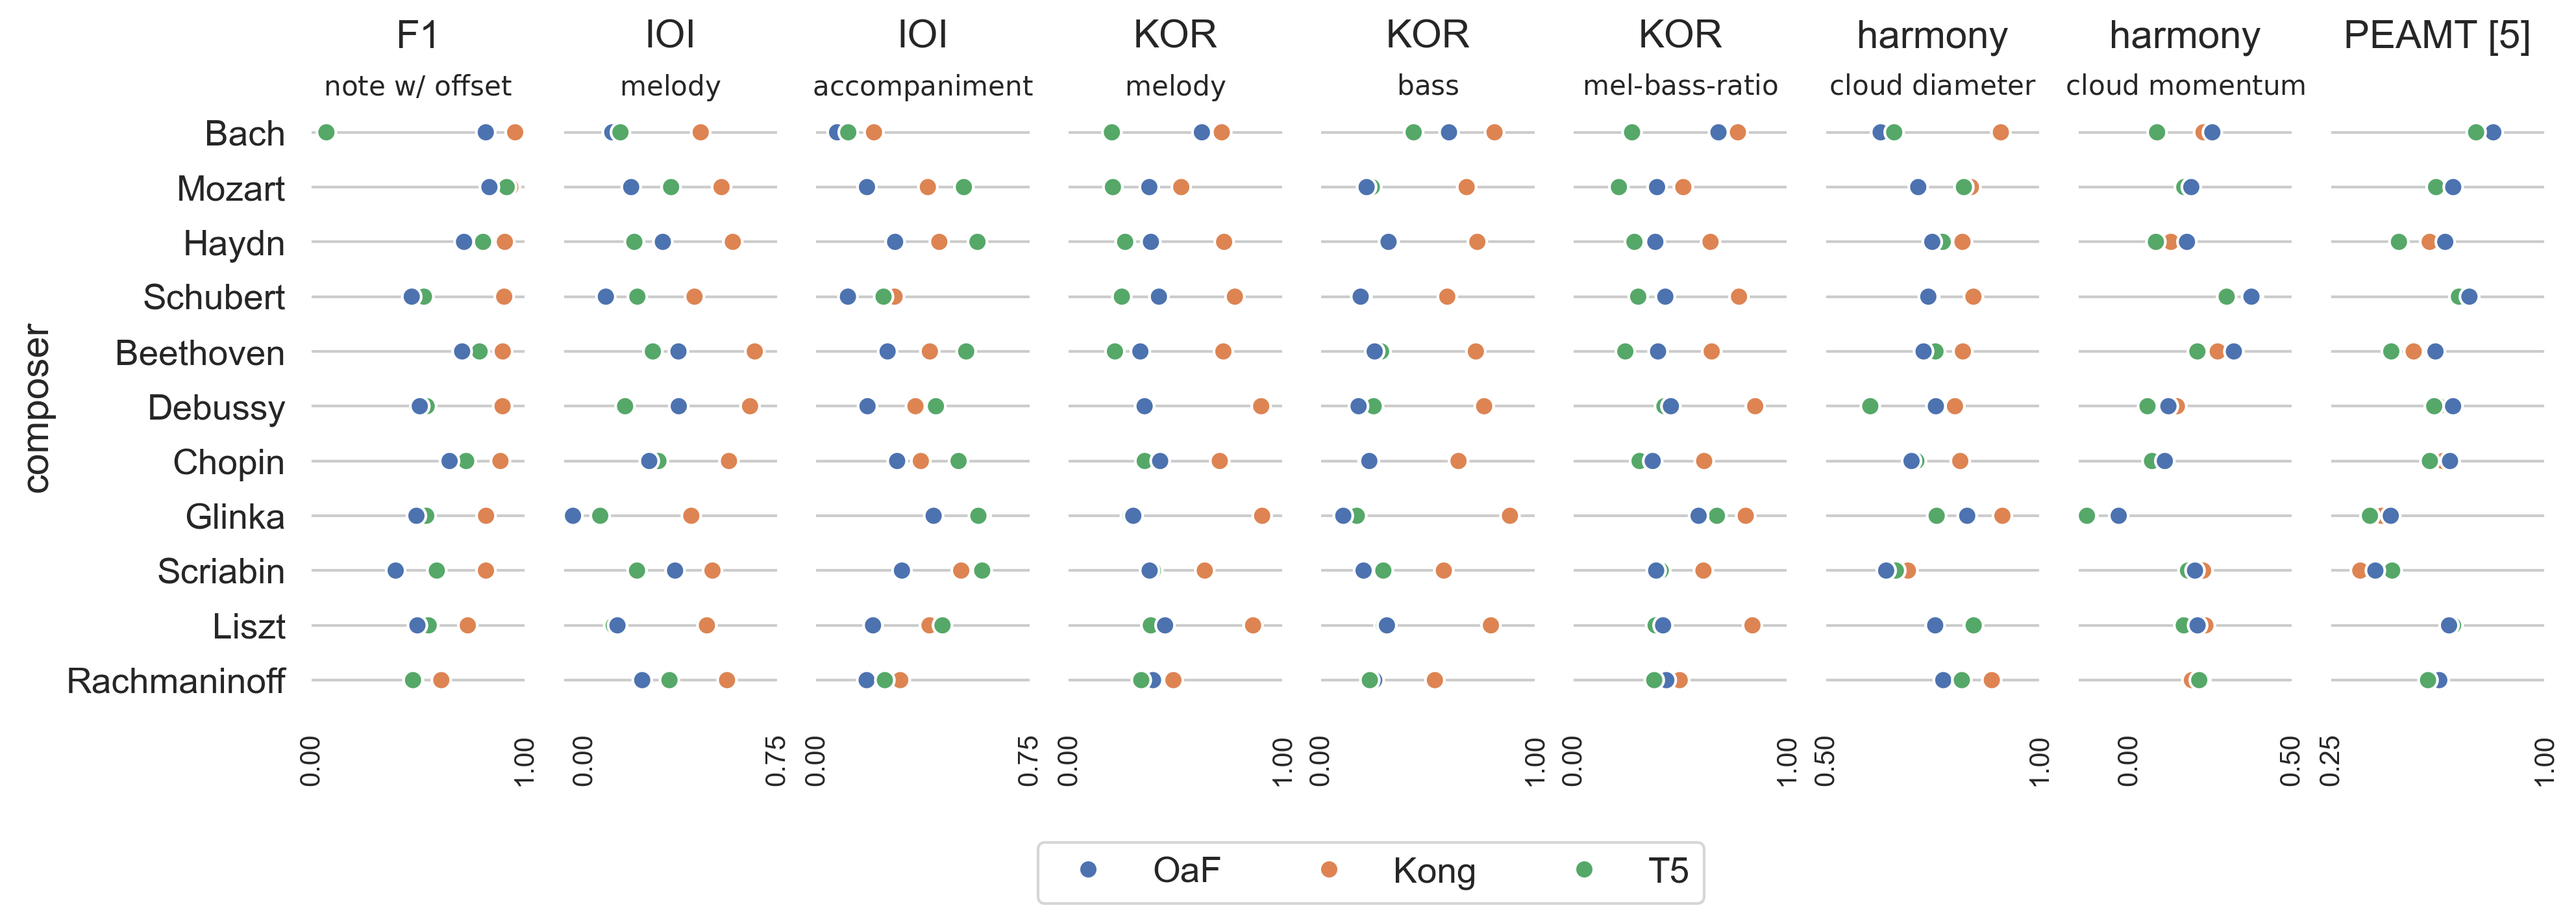
\includegraphics[width=\textwidth]{assets/figs/exp1_IR-vs-music_metrics_composer_split_height=4_whitegrid_xticks_90.png}
  \caption{Model performance comparison as evaluated on note-offset F1 score and our proposed musical metrics, by composer.}
  \label{fig:composerwise_MAESTRO}
\end{figure*}

\section{Demonstration of musically informed metrics}\label{sec:demonstration}

We now discuss the experimental results obtained with the three systems and explain the relation between our metrics and the standard IR metrics as computed on transcriptions of the MAESTRO subset of our \textit{evaluation set}. We focus in particular on the musical dimensions that can be better understood through our metrics. For the standard evaluation, we include the frame-level score, and all note-level F1 scores other than the onset-only as they do not capture offset and velocity information. We compute the note-level metrics with the official \texttt{mir\_eval} python implementation \cite{raffel2014mir_eval}.

We start our discussion with Table \ref{tab:maestro_all_metrics_res}, which summarizes the evaluation results per model and metric. % on all MAESTRO recordings in our \textit{evaluation set}. 
For comparative reasons, we also include a perceptually informed piano transcription metric, PEAMT \cite{ycart2020investigating}.

\begin{table}[ht]%[hbt!]
    % \small
    \centering
    \input{tables/exp1_all_metrics_res_MAESTRO}
    \captionsetup{width=.95\columnwidth}
    \caption{Performance of the three models using the standard metrics, our musically informed metrics, and the perceptually informed PEAMT metric \cite{ycart2020investigating} as computed on the MAESTRO subset of our \emph{evaluation set}.}
    \label{tab:maestro_all_metrics_res}
\end{table}

Generally, it can be observed that the Kong model performs the best across most metrics. This implies that most of our metrics, overall, correlate with the performance ranking as measured on the standard metrics. 
Furthermore, it can be seen that the two Magenta models perform significantly different when measured against frame-level F1 score, yet this difference becomes less pronounced when evaluated on note-level metrics, which would suggest superior performance of the T5 model. Comparing these results to the model performance as evaluated on our set of metrics, however, reveals that while both models perform similarly on onset time prediction, the T5 model is worse at adequately capturing note durations, particularly in lower voices/frequency ranges, but superior in estimating MIDI velocity and the overall loudness ratio between voices than the OaF model.
% Lukas @ Paty: The observation below stems from your correlation plot (not present in the paper), or from the table 2? Maybe the actual correlations visualized somehow might be useful too in a future version 
Lastly, we can observe that the perceptually informed PEAMT metric correlates most with the frame-level and harmony metric \emph{Cloud Momentum}, which might suggest (if PEAMT is indeed a veridical listening model) that listeners place relatively high importance on harmonic context.

\begin{figure}[ht]%[hbt!] 
  \includegraphics[width=0.95\columnwidth]{figs/dynamics_vs_note_offset_velocity.pdf}
  \captionsetup{width=.95\columnwidth}
  \caption{Relationship between model performance evaluated on note-offset-velocity F1 score and our proposed dynamics measure.}
  \label{fig:dynamics_vs-fnov}
\end{figure}


% TODO: Replace this with a figure that visually conveys the message more starkly
\begin{table*}[b!]%[bp]
    \small
    \centering
    \input{tables/exp2_eval_benchmark_note-frame}
    \captionsetup{width=.95\textwidth}
    \caption{Frame-, note-offset, and note-offset-velocity F1 score results computed on our \emph{\textit{evaluation set}}, grouped per data set split, evaluated model and piano / audio environment.}
    \label{tab:eval_benchmark_results}
\end{table*}


We continue our discussion in Figure \ref{fig:composerwise_MAESTRO}, which compares the note-offset F1 score per composer (averaged over pieces and performers) and model to our musically informed timing, articulation and harmony metrics. We can see again that the Kong model performs best across all composers and metrics except for the \emph{Accompaniment IOI} timing and the \emph{cloud momentum} harmony metrics. The fact that it performs better on the \emph{Bass KOR} articulation metric, but poorly on those timing accompaniment and harmony metrics might suggest that this model detects many out-of-key extra notes that both erroneously influences the IOI sequence on the accompaniment part, and the estimation of the tonal context. Interestingly, we can can also observe, as a general trend, that the F1 score somewhat deteriorates with increasing virtuoso and challenging musical repertoire. This general deterioration with increasing musical difficulty is not reflected correspondingly by our metrics, which show more variation with respect to different composers and aspects of the underlying music: While the F1 score for Bach, Mozart, Haydn and Schubert all suggest a near-perfect transcription, our metrics indicate more diverse results, and e.g., suggest poor(er) accuracy (and therefore reliability in a performance study context) in the \emph{Melody IOI} and \emph{Melody KOR} metrics. Another illustrative example can be found in the case of Chopin: here again the F1 score (particularly of the Kong model) would suggest a highly accurate transcription output, while our metrics reveal that the expressive dimension of articulation is not well captured. Lastly, we can observe again that the PEAMT and harmony metric \emph{Cloud momentum} show a similar trend for most composers, suggesting a greater weight of the harmonic context in that trained metric.

We conclude our discussion by examining the dynamics aspect. Figure \ref{fig:dynamics_vs-fnov} illustrates the relationship between the note-offset-velocity F1 score and our proposed \emph{dynamics} metric. While both metrics show a weak correlation (Pearson $r=0.21$), the figure also indicates that our metric evaluates dynamics in a more differentiated way and leads to a wider range of evaluation results than the standard metric. Note that our metric only evaluates the dynamics aspect, in particular how well the overall balance in loudness between different voice streams is preserved in a transcription. It does not account for onset, offset and pitch information, which also explains the results in the very left part of the figure that score low on F1 score but high on our metric.


\section{Out-of-distribution inference}\label{sec:ood_inference}

In this section we illustrate the problem of out-of-distribution performance of the models analysed. We believe that this is an important aspect to emphasize, as transcription models are ultimately intended to be (and have been) used on real-world audio performances \cite{kong2020giantmidi, zhang2023atepp}. 

We approach the problem in two stages: First, we elucidate the problem by performing a short evaluation of the three analysed models on real-world recordings using only the standard IR metrics. Second, we simulate more challenging real-world environments using different levels of noise and reverberation, and evaluate the analysed models again using the standard and our proposed metrics, where we highlight how our musically informed metrics can reveal aspects that the standard metrics would otherwise have missed.

% h 	Place the float here, i.e., approximately at the same point it occurs in the source text (however, not exactly at the spot)
% t 	Position at the top of the page.
% b 	Position at the bottom of the page.
% p 	Put on a special page for floats only.
% ! 	Override internal parameters LaTeX uses for determining "good" float positions.
% H 	Places the float at precisely the location in the LaTeX code. Requires the float package. This is somewhat equivalent to h!. 

\subsection{Generalization on real-world recordings}

Table \ref{tab:eval_benchmark_results} shows the mean frame- and note-level F1 scores per model and per piano/acoustic recording environment on the three splits of the MAESTRO dataset (as they are officially defined).\footnote{We note that for the two Magenta models, OaF and T5, our evaluation results do not come close to the reported ones in \cite{hawthorne2019enabling} and \cite{hawthorne2021sequence}. The differences are particularly pronounced in the note-level F1 scores.}


% model  |  frame  |  note_on  | note_on_off  |  note_on_off_vel
% OAF    |  90.15  |    95.32  |    80.50     |     77.54
% OaF r  |  85.27  |    -      |    59.31     |     56.95
% Kong   |  98.62  |    96.72  |    82.47     |     80.92
% Kong r |  90.02  |    -      |    82.15     |     80.41
% T5     |    -    |    96.01  |    83.94     |     82.75
% T5 r   |  65.52  |    -      |    59.68     |     58.96

% model  |  frame  | note_on   | note_on_off  |  note_on_off_vel
% OAF    |  90.15  |    95.32  |    80.50     |     77.54
% Kong   |  98.62  |    96.72  |    82.47     |     80.92
% T5     |    -    |    96.01  |    83.94     |     82.75

% and on the \textit{Batik} evaluation subset. 

We group the results per split to test whether the analysed models would perform worse on out-of-distribution recordings of performances (pieces) from the test set compared to those from the train/validation sets.
% \gw{This "split" business thoroughly confused me for a while. Please explicitly explain here that (if I got this right now) the "three splits" you are talking about here are defined by the original MAESTRO dataset, and that - since your \textit{evaluation set} contains pieces from all of the three splits (which you explained as "purposefully done" somewhere above), you can do this. Why do you do the analysis by splits now? what do you want to see?} 
Next we conduct a Kruskal Wallis ANOVA\cite{vargha1998kruskal} to test for differences between frame-, note-offset and note-offset-velocity F1 scores, grouping the evaluation scores each by \textit{split} and by \textit{audio environment} and comparing each model separately. For each ANOVA we use a significance threshold of $\alpha=0.05$. The ANOVA on the \textit{audio environment} dimension show a statistically significant difference ($p<0.05$) between the MAESTRO and Disklavier audio recordings for all three analysed models.

The ANOVA on the \textit{split} dimension yields more differentiated results:  For all models, the frame-level F1 scores are significantly different, and there are no statistically significant differences in the note-offset-velocity F1 scores. For the model by Kong, the note-offset-score is significantly different depending on the split, whereas the two Magenta models show no significant differences. This suggests that the most musically meaningful metric from the current set of standard metrics\cite{hawthorne2017onsets} does not sufficiently capture overfitting tendencies.

% stats results:
%{

% -- grouped by split
% > OaF : frame-f are different but note-offset and note-offset-vel are same
% > kong : frame-f and note-offset are different but note-offset-vel are same 
% > T5 : frame-f are different but note-offset and note-offset-vel are same

% -- grouped by audio environment 
% > OaF : all f scores are different
% > kong : all f scores are different
% > T5 : all f scores are different
% }

\subsection{Evaluation on perturbed audio recordings}

Similar as in Section \ref{sec:demonstration}, we again compare our musically informed metrics to the standard IR and the PEAMT metrics, however, this time on a set of more challenging audio recordings. To this end, we choose six (MAESTRO and \textit{Disklavier}) audio recordings which we artificially perturb by introducing reverberation and synthetic noise. 
We use three Impulse-Response filters, modelling short, medium and long reverberation times (RT60@1kHz $\in \{0.19, 1.85, 10.5\}$ seconds) and sourced from the OpenAIR\footnote{\url{https://www.openair.hosted.york.ac.uk}} database.
%The selected IR filters are modelling a i) studio room\footnote{\url{https://www.openair.hosted.york.ac.uk/?page_id=483}} ii) concert hall\footnote{\url{https://www.openair.hosted.york.ac.uk/?page_id=571}}; and iii) a factory warehouse\footnote{\url{https://www.openair.hosted.york.ac.uk/?page_id=735}}. 
We further add white noise into the recordings at three different Signal-to-Noise Ratio levels ($\text{SNR}_{dB} \in \{24, 12, 6\}$).
Following a factorial design with these two independent variables, each with four levels, we first perturb the audio recordings on all conditions, and transcribe these recordings using all three analysed models. Following this procedure, we obtain 284 transcribed MIDI performances.\footnote{Note that 6 pieces x 4 noise levels x 4 reverberation levels x 3 models yield 288 transcriptions, but 4 recordings (each at the two higher most of either reverberation and/or noise levels) resulted in empty transcriptions (zero predicted note events) by the T5 model, and are therefore excluded from the evaluation.}

Each grid cell in Figure \ref{fig:exp2_revnoise_fig} compares the mean note-offset F1 scores per model to the \emph{Melody IOI} timing metric and \emph{cloud momentum} harmony metric, where grid rows represent increasing reverb levels, and grid columns represent increasing noise levels.
Generally, it can be observed that the performance range of models as measured by the F1 score is notably reduced compared to our metrics, indicating that our metrics possess higher discriminative capacity than the standard ones.

As expected, the inference performance of all three analysed models deteriorates with increasing noise and reverberation levels, though the deterioration is less pronounced on the noise than on the reverberation axis. 
Furthermore, analysing the results on the timing metric \emph{Melody IOI} suggests that the model by Kong predicts onset times worse with increasing noise levels, while the onset times prediction by OaF seems to be more resistant to this form of perturbation. Finally, the results measured on the harmony metric \emph{Cloud momentum} suggest that the overall harmonic context is relatively well preserved at higher perturbation levels by the OaF and Kong models, and less so by the T5 model.

\begin{figure}[t]%[hbt!] 
  \includegraphics[width=0.95\columnwidth]{figs/exp2_revnoise.pdf}
  \captionsetup{width=1\columnwidth}
  \caption{Performance degradation analysis as evaluated on the note-offset F1 score and our proposed \emph{Melody IOI} timing and \emph{Cloud momentum} harmony metric.}
  \label{fig:exp2_revnoise_fig}
\end{figure}

\section{Conclusion}\label{sec:conclusion}

In this study, we investigated two aspects that are commonly neglected in the evaluation of transcription models: (i) limited explanatory power of the standard IR evaluation metrics with respect to the underlying musical material, and (ii) poor inference on out-of-distribution data. We study both problems in the context of solo piano transcription, and, in addressing the first aspect, propose a set of musically informed metrics designed to capture more musically relevant information, particularly for the context of computational studies of expressive performance.

We demonstrated our metrics on transcriptions obtained by three state-of-the-art piano transcription models on a subset of the MAESTRO dataset, the de-facto standard train and test set for current transcription models, and highlighted musical dimensions for which they provide more informative value than the standard information retrieval metrics.
% by which transcription models are otherwise evaluated. 
We have further illustrated the lack of generalization with respect to the acoustic environment, both on real-world and perturbed audio recordings. We plan to extend our musically informed metrics to capture more qualities of expressive performance, possibly using score alignment information.

% Our plans for future work include an extension of our musically informed metrics to capture more qualities of expressive performance, potentially by making use of score alignment information. 
% Furthermore, we plan to conduct a listening test to evaluate the perceptual validity of our proposed metrics.
% We plan to extend our musically informed metrics to capture more qualities of expressive performance, possibly using score alignment information. Additionally, we will conduct a listening test to evaluate the perceptual validity of these metrics.

\section{Acknowledgments} 
This work receives funding from the European Research Council (ERC), under the European Union's Horizon 2020 research and innovation programme, grant agreement No.~101019375 (\textit{Whither Music?}). The LIT AI Lab is supported by the Federal State of Upper Austria.

% \section{Ethics Statement} OPTIONAL

% For bibtex users:
\bibliography{ISMIRtemplate}


\end{document}

